\documentclass{beamer}
\beamertemplatenavigationsymbolsempty
\usecolortheme{beaver}
\setbeamertemplate{blocks}[rounded=true, shadow=true]
\setbeamertemplate{footline}[page number]
%
\usepackage[utf8]{inputenc}
\usepackage[english, russian]{babel}
\usepackage{amssymb,amsfonts,amsmath,mathtext}
\usepackage{subfig}
\usepackage[all]{xy} % xy package for diagrams
\usepackage{array}
\usepackage{multicol}% many columns in slide
\usepackage{hyperref}% urls
\usepackage{hhline}%tables
\usepackage{algorithm}
\usepackage{algpseudocode}
\usepackage{amsmath}
\usepackage{tikz}
\usetikzlibrary{positioning}
\usepackage{amssymb}
\usepackage{array}
\renewcommand{\arraystretch}{2} % увеличение отступа между строками
\usepackage{dashbox}
\usepackage[most]{tcolorbox}


\setlength{\columnsep}{1cm}

\usepackage{setspace}

\newcommand{\advisor}[1]{\gdef\@advisor{#1}}
\newcommand{\printadvisor}{\@ifundefined{@advisor}{}{\textbf{Advisor:} \@advisor}}

\newcommand{\supervisor}{}


% Your figures are here:
\graphicspath{{./figures}}

%----------------------------------------------------------------------------------------------------------
\title[\hbox to 56mm{Feature generation}]{On the Dirichlet Prior and Bayesian Regularization}
\author[~Babkin]{Бабкин Пётр}
\institute{}
\date{}

%----------------------------------------------------------------------------------------------------------
\begin{document}
%----------------------------------------------------------------------------------------------------------
\begin{frame}
    \thispagestyle{empty}
    \maketitle
    \vspace{-2.3cm}
    \centering
    
    \vspace{0.6cm}

\bigskip

2024

\end{frame}

%----------------------------------------------------------------------------------------------------------
\begin{frame}{Bayesian Network}

    \begin{columns}[c]
    \column{0.4\textwidth}

        \begin{tikzpicture}[
            roundnode/.style={circle, draw=gray!60, fill=gray!5, very thick, minimum size=7mm},
            ]
            %Nodes
            \node[roundnode]      (one)                              {$\Pi_1$};
            \node[roundnode]        (two)       [below=of one] {$\Pi_2$};
            \node[roundnode]      (three)       [right=of one] {$X$};
            
            %Lines
            \draw[->] (one.east) -- (three.west);
            \draw[->] (two.east) -- (three.south);
            \draw[->] (two.north) -- (one.south);
            \end{tikzpicture}
       
    \column{0.6\textwidth}

        $$ p(x, \pi_1, \pi_2) = p(\pi_2) p(\pi_1 | \pi_2) p(x | \pi_1, \pi_2) $$
        
    \end{columns}

    \bigskip
    \bigskip
    $$p(D) = \prod_{x_i} p(x_i | \pi_i) \quad \quad i = 1, \ldots, n$$

    \bigskip

    $X \sim $ discrete distribution with probability vector $\{ \theta_{x_i, \pi_i} \}$

    $N_{x_i, \pi_i} = $number of realizations
    
    $\{N_{x_i, \pi_i}\} \sim Mult(\{ \theta_{x_i, \pi_i} \})$
    
    \bigskip
    
    
\end{frame}

%----------------------------------------------------------------------------------------------------------
\begin{frame}{Dirichlet Prior and Regularization of Parameters}

\begin{block}{Prior}
$$p(\theta_{X_i | \pi_i}) = \frac{1}{B(\alpha_{X_i, \pi_i})} \prod_{x_i} \theta^{\alpha_{x_i, \pi_i} - 1}_{x_i | \pi_i} $$

$\quad \sum_{x_i, \pi_i} \alpha_{x_i, \pi_i} = \alpha $ -- scale parameter
\end{block}

\begin{block}{Likelihood}
$$N_{X_i, \pi_i} | \theta_{X_i, \pi_i} \sim Mult(\theta_{X_i, \pi_i})$$
\end{block}

\begin{block}{Posterior}
$$\theta_{X_i, \pi_i} | N_{X_i, \pi_i} \sim Dir(\alpha_{X_i, \pi_i} + N_{X_i, \pi_i})$$
\end{block}


with $\alpha \to 0, \quad \theta_{X_i, \pi_i} \to MLE$

\end{frame}
%----------------------------------------------------------------------------------------------------------
\begin{frame}{Regularization of Structure}

\begin{block}{Prior}
$$p(m) > 0 \quad \forall m$$
\end{block}

\begin{block}{Posterior}
$$p(m | D) = \frac{p(D | m) p(m)}{p(D)}$$
\end{block}

\begin{block}{Marginal Likelihood}
$$p(D | m) = \int p(D | m, \theta) p(\theta | m) d\theta = \prod_{k=1}^{N} \prod_{i=1}^{n} \frac{N^{k-1}_{x_i^k, \pi_i^k} + \alpha_{x_i^k, \pi_i^k}}{N^{k-1}_{\pi_i^k} + \alpha_{\pi_i^k}} $$
\end{block}


with $\alpha \to 0, \quad \theta_{X_i, \pi_i} \to MLE$

\end{frame}
%----------------------------------------------------------------------------------------------------------
\begin{frame}{Limit of Vanishing Scale-Parameter}
    \begin{tcolorbox}[
    colback=gray!10, colframe=gray!50, arc=5mm,
    boxsep=0.5mm, left=3mm, right=3mm, top=2mm, bottom=2mm
    ]
    \textbf{Proposition 1.}\quad The marginal likelihood of a Bayesian network structure $m$ vanishes in the limit $ \alpha \to 0$ if the data D contain two or more different configurations.
    
    The leading polynomial order is given by
    \begin{equation*}
          p(D|m) \sim \alpha^{d_{EP}^{(m)}} \quad as \quad \alpha \to 0.
    \end{equation*}
    \end{tcolorbox}
    $$d_{EP}^{(m)} = \sum_i\left(\sum_{x_i, \pi_i} \mathbf{I}(N_{x_i, \pi_i}) - \sum_{\pi_i}\mathbf{I}(N_{\pi_i})\right)$$

\end{frame}
%----------------------------------------------------------------------------------------------------------
\begin{frame}{Vanishing Graph}

    Let edge $A \to B \in m^+$ and $A \to B \notin m^-$

    $$d_{EDF} = d_{EP}^{m_+} - d_{EP}^{m_-}$$

    \begin{tcolorbox}[
    colback=gray!10, colframe=gray!50, arc=5mm,
    boxsep=0.5mm, left=3mm, right=3mm, top=2mm, bottom=2mm
    ]
    \textbf{Proposition 2.} \quad In the limit $\alpha \to 0$:
    
    \begin{equation*}
          \log \frac{p(D | m^+)}{p(D | m^-)} = \begin{cases}
              -\infty & d_{EDF} > 0 \\
              +\infty & d_{EDF} < 0
          \end{cases}
    \end{equation*}
    \end{tcolorbox}
    Proposition is applicable to any edge in the graph.
    
    \bigskip
    
    Empty (complete) graph is assigned the highest relative Bayesian score when EDF are positive (negative).

    Positive (negative) EDF relates to large (small) dataset.

\end{frame}
%----------------------------------------------------------------------------------------------------------
\begin{frame}{Large Scale-Parameter and Example}

    $$\log\frac{p(D | m^+)}{p(D | m^-)} \to 0 \quad as \quad \alpha \to \infty $$

    \begin{figure}
        \centering
        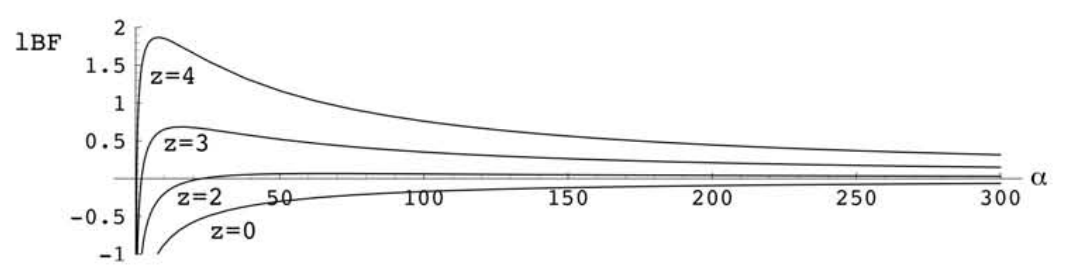
\includegraphics[width=0.8\textwidth]{figures/lBF-alpha.png}
    \end{figure}

    As $\alpha \to \infty$, edges with weak connections are favored over no connections. 

\end{frame}
%----------------------------------------------------------------------------------------------------------
\begin{frame}{Trade-off}

\textit{Hence, the scale parameter $\alpha$: of the Dirichlet prior
determines the trade-off between regularizing the parameters vs the structure of the Bayesian network model.}

\end{frame}
%----------------------------------------------------------------------------------------------------------
% \begin{frame}{Литература}
%     \begin{itemize}
%         \setlength\itemsep{1.3em}
%         \item Yao Shu1, Yizhou Chen, Zhongxiang Dai, Bryan Kian, Hsiang Low: \href{https://arxiv.org/pdf/2109.02533.pdf}{\textcolor{blue}{Neural Ensemble Search via Bayesian Sampling}}
%         \item Hanxiao Liu, Karen Simonyan, Yiming Yang: \href{https://arxiv.org/pdf/1806.09055.pdf}{\textcolor{blue}{DARTS: Differentiable Architecture Search}}
%         \item Konstantin Yakovlev, Olga Grebenkova, Oleg Bakhteev, Vadim Strijov: \href{https://easychair.org/publications/preprint/H5MC}{\textcolor{blue}{Neural Architecture Search with Structure Complexity Control}}
%         \item Ashwin Raaghav Narayanan, Arber Zela, Tonmoy Saikia, Thomas Brox, Frank Hutter: \href{https://arxiv.org/pdf/2107.04369.pdf}{\textcolor{blue}{Multi-headed Neural Ensemble Search}}
%     \end{itemize}
% \end{frame}
%----------------------------------------------------------------------------------------------------------
\end{document} 